%==============================================================================
% Sjabloon onderzoeksvoorstel bachproef
%==============================================================================
% Gebaseerd op document class `hogent-article'
% zie <https://github.com/HoGentTIN/latex-hogent-article>

% Voor een voorstel in het Engels: voeg de documentclass-optie [english] toe.
% Let op: kan enkel na toestemming van de bachelorproefcoördinator!
\documentclass{hogent-article}

% Invoegen bibliografiebestand
\addbibresource{voorstel.bib}

% Informatie over de opleiding, het vak en soort opdracht
\studyprogramme{Professionele bachelor toegepaste informatica}
\course{Bachelorproef}
\assignmenttype{Onderzoeksvoorstel}
% Voor een voorstel in het Engels, haal de volgende 3 regels uit commentaar
% \studyprogramme{Bachelor of applied information technology}
% \course{Bachelor thesis}
% \assignmenttype{Research proposal}

\academicyear{2022-2023} % TODO: pas het academiejaar aan

% TODO: Werktitel
\title{Implementatie van GraphQL binnen een zelfontwikkelde accelerator}

% TODO: Studentnaam en emailadres invullen
\author{Bram Stevens}
\email{bram.stevens@student.hogent.be}

% TODO: Medestudent
% Gaat het om een bachelorproef in samenwerking met een student in een andere
% opleiding? Geef dan de naam en emailadres hier
% \author{Yasmine Alaoui (naam opleiding)}
% \email{yasmine.alaoui@student.hogent.be}

% TODO: Geef de co-promotor op
\supervisor[Co-promotor]{Simon Dedeken (Delaware, \href{mailto:simon.dedeken@delaware.pro}{simon.dedeken@delaware.pro})}

% Binnen welke specialisatierichting uit 3TI situeert dit onderzoek zich?
% Kies uit deze lijst:
%
% - Mobile \& Enterprise development
% - AI \& Data Engineering
% - Functional \& Business Analysis
% - System \& Network Administrator
% - Mainframe Expert
% - Als het onderzoek niet past binnen een van deze domeinen specifieer je deze
%   zelf
%
\specialisation{Databanken en big-data}
\keywords{GraphQL, Accelerator, Microsoft Azure}

\begin{document}

\begin{abstract}
GraphQL (Graph Query Language) staat al reeds enkele jaren gekend als een open-source data query computertaal ten dienste van API's. Deze wordt sinds zijn vrijgeving een aantal jaren geleden, steeds uitgebreider en door meer en meer bedrijven geïmplementeerd. Bij IT- en businessconsultingbedrijf Delaware wordt zich nu de vraag gesteld of dit opportuniteiten kan bieden, in samenwerking met een zelfontwikkeld accelerator-systeem dat Data Accelerator heet. Dit heeft als gevolg dat er een onderzoek naar een mogelijke implementatie of integratie genoodzaakt is. Het doel is om na te gaan hoe deze twee technologieën samen kunnen werken en of er mogelijke alternatieven zijn.
\end{abstract}

\tableofcontents

% De hoofdtekst van het voorstel zit in een apart bestand, zodat het makkelijk
% kan opgenomen worden in de bijlagen van de bachelorproef zelf.
%---------- Inleiding ---------------------------------------------------------

\section{Introductie}%
\label{sec:introductie}

Meta, voormalig gekend als facebook, ontwikkelde in 2012 een query computertaal genaamd GraphQL om een intern probleem op te lossen. Deze werd in 2015 publiek gesteld en nam sindsdien enorm aan populariteit toe. Veel gekende bedrijven zoals Airbnb, Audi, GitHub, KLM, NBC, PayPal en nog vele anderen gebruiken de computertaal ondertussen al. Ook bij Delaware groeit nu de interesse om zich te verdiepen in GraphQL en de toepassingen die deze technologie met zich meedraagt, rekeninghoudend of dit voor hun een opportuniteit biedt om hun software te verbeteren. In het onderzoek zal dan ook aan bod komen wat die opportuniteiten juist inhouden. Delaware ontwikkelde zelf ook een accelerator die als benaming “Data Accelerator“ kreeg. Wat deze exact doet zal verder uitgelegd worden in sectie 2 - Literatuurstudie.

Vanwege de mogelijke voordelen die een implementatie of integratie van GraphQL met de Data Accelerator kan bieden, wordt dit dus ook het grondthema van deze bachelorproef. Dit op zijn beurt zal theoretisch benaderd worden met als doel naar verloop een fysiek resultaat op te leveren. Deze opzet kan beschreven worden met de volgende onderzoeksvraag: ''Hoe kan GraphQL geïmplementeerd worden in een zelfontwikkelde accelerator?''

Het oogmerk van dit onderzoek is reeds beschreven in de onderzoeksvraag. Echter om deze te behalen moeten de volgende deelvragen beantwoord geraken: \newline - Wat is GraphQL?\newline - Wat is een (Data) Accelerator?\newline - Kan Data Accelerator GraphQL benutten?\newline - Welke integratie mogelijkheden zijn er voor GraphQL binnen Data Accelerator?

Het mikpunt van dit onderzoek is om zo snel mogelijk een concreet voorbeeld te kunnen bieden. Dit is zichtbaar aan de volgorde van de hierbovenstaande deelvragen die opgelijst zijn.


%---------- Stand van zaken ---------------------------------------------------

\section{Literatuurstudie}%
\label{sec:Literatuurstudie}

\subsection{Wat is GraphQL?}
Graph Query Language beter gekend als GraphQL is een query computertaal. Deze maakt gebruik van een API om niet zelf rechtstreeks de data te behandelen. GraphQL brengt een zelfde resultaat tot stand als soortgelijke software, maar op een verschillende manier. Namelijk, de aanvragen worden anders opgebouwd zodat juist de benodigde data ter beschikking komt. De computertaal werd ontwikkeld in 2012 door facebook uit noodzaak tijdens hun converteren naar hun native apps, voorheen mobile apps,
in dienst van hun mobiele website. Soortgelijke software kon hun vereisten niet voldoen vanwege de grote disproportie tussende data en de hoeveelheid server queries die nodig waren. Facebook zocht naar een manier om queries die serverdata collecteren gelijkend te maken aan de samenstelling van hun data. Op deze manier kon er gerichter gewerkt worden om juist de benodigde data ter beschikking te stellen \autocite{Brysbaert2021}.

\subsection{(Data) Accelerator}
Accelerators kunnen gedefinieerd worden als een inhoud bevattende verzameling die inspelen op een vaak voorkomend probleem rondom data kwaliteit. Dit zal vaak in functie van een geografisch gebied of een type van industrie zijn. Deze kan aan de hand van herbruikbare objecten of gespecifieerde regels data analyseren en uitbreiden binnenin een bedrijf. Mogelijks kan deze ook over data domeinen beschikken om verschillende types van info die de data bevat te ontdekken\newline\autocite{Informatica2021}.

Binnenin het computerlandschap zijn er vaak transities van homogene naar heterogene knooppunten. Dit wil zeggen dat in plaats van eenzelfde functie deze gecategoriseerd worden naar gelang hun functie. Dit kan u best vergelijken met het verschil tussen een koper en een verkoper van schoenen. Accelerators kunnen in functie staan van een grafische processor, computerchips die over meerdere kernen beschikken, schakelingen van logische componenten of een microprocessor om digitale signalen te bewerken. Hier is hun doel dan om taken die heel reken-intensief zijn, te lichten voor het systeem \autocite{LopezNovoa2015}.

De accelerator die in gebruik gesteld wordt van Delaware in functie van dit onderzoek zal verder uitgespit worden in deze bachelorproef zodat er een duidelijk gedefinieerde basis is waaruit er vertrokken wordt.

%---------- Methodologie ------------------------------------------------------
\section{Methodologie}%
\label{sec:methodologie}

Om de opgelijste deelvragen te kunnen beantwoorden is er een literatuurstudie nodig als startpunt. Daarom is dit dus ook de eerste fase van het onderzoek. In de literatuurstudie kan het volgende nagekeken worden:\newline Wat is de exacte werking van GraphQL en hoe implementeerd of integreert men dit?\newline Welke opportuniteiten of nadelen kan GraphQL opleveren?\newline Kan men GraphQL integreren in een accelerator of moet men implementeren? \newline Wat is de complexiteit van de uit te voeren integratie of implementatie?

Hiervoor wordt er een case study uitgevoerd die kan nagaan welke oplossing juist het meest voordelig is en of Microsoft Azure al dan niet soortgelijke implementaties reeds bevat. Zo kunnen we nagaan of deze implementatie nodig is of op een andere manier bereikt kan worden.

%---------- Verwachte resultaten ----------------------------------------------
\section{Verwachte resultaat}
\label{sec:verwachte resultaat}
Het verwachte resultaat van deze case study moet een praktische oplossing zijn voor de implementatie van GraphQL. Dit moet een overzicht kunnen leveren aan lezers die zich willen verdiepen in deze kwestie. Voor Delaware moet het mogelijk zijn om evenals een duidelijk stappenplan te verkrijgen om dit dan effectief ook uit te voeren indien gewenst. De mogelijke alternatieve oplossingen binnen Azure zouden hier dan ook aangekaart worden.

\section{Verwachte conclusie}
\label{sec:verwachte conclusiet}
Als echter vele bedrijven reeds de stap zetten en gebruikmaken van GraphQL is dit voor Delaware ook interessant om te zien welke mogelijke toepassingen er allemaal zijn die in hun voordeel spelen. Er is een grote kans dat het mogelijk is om GraphQL en Data Accelerator samen te laten werken via integratie of implementatie. Evenals is het niet ondenkbaar dat Microsoft Azure functies bevat waarvoor het onnodig kan zijn wegens betere alternatieven.


\chapter{bijlagen}

\section{Workflow}%
\label{sec:Workflow}
\begin{figure}[H]
    \centering
    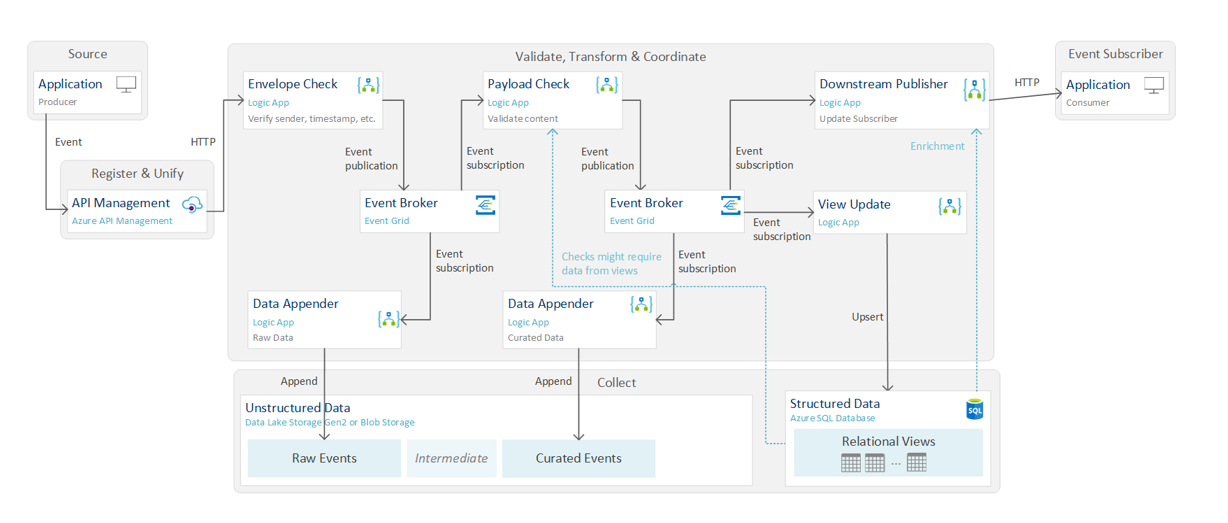
\includegraphics[]{img/Workflow.PNG}
\end{figure}



\printbibliography[heading=bibintoc]

\end{document}